% !TEX root = ../main.tex

\begin{frame}{Audio Mixer Controls: Layers}
	\begin{columns}[T,onlytextwidth]
		\column{0.6\textwidth}
		\begin{figure} 
			\centering
			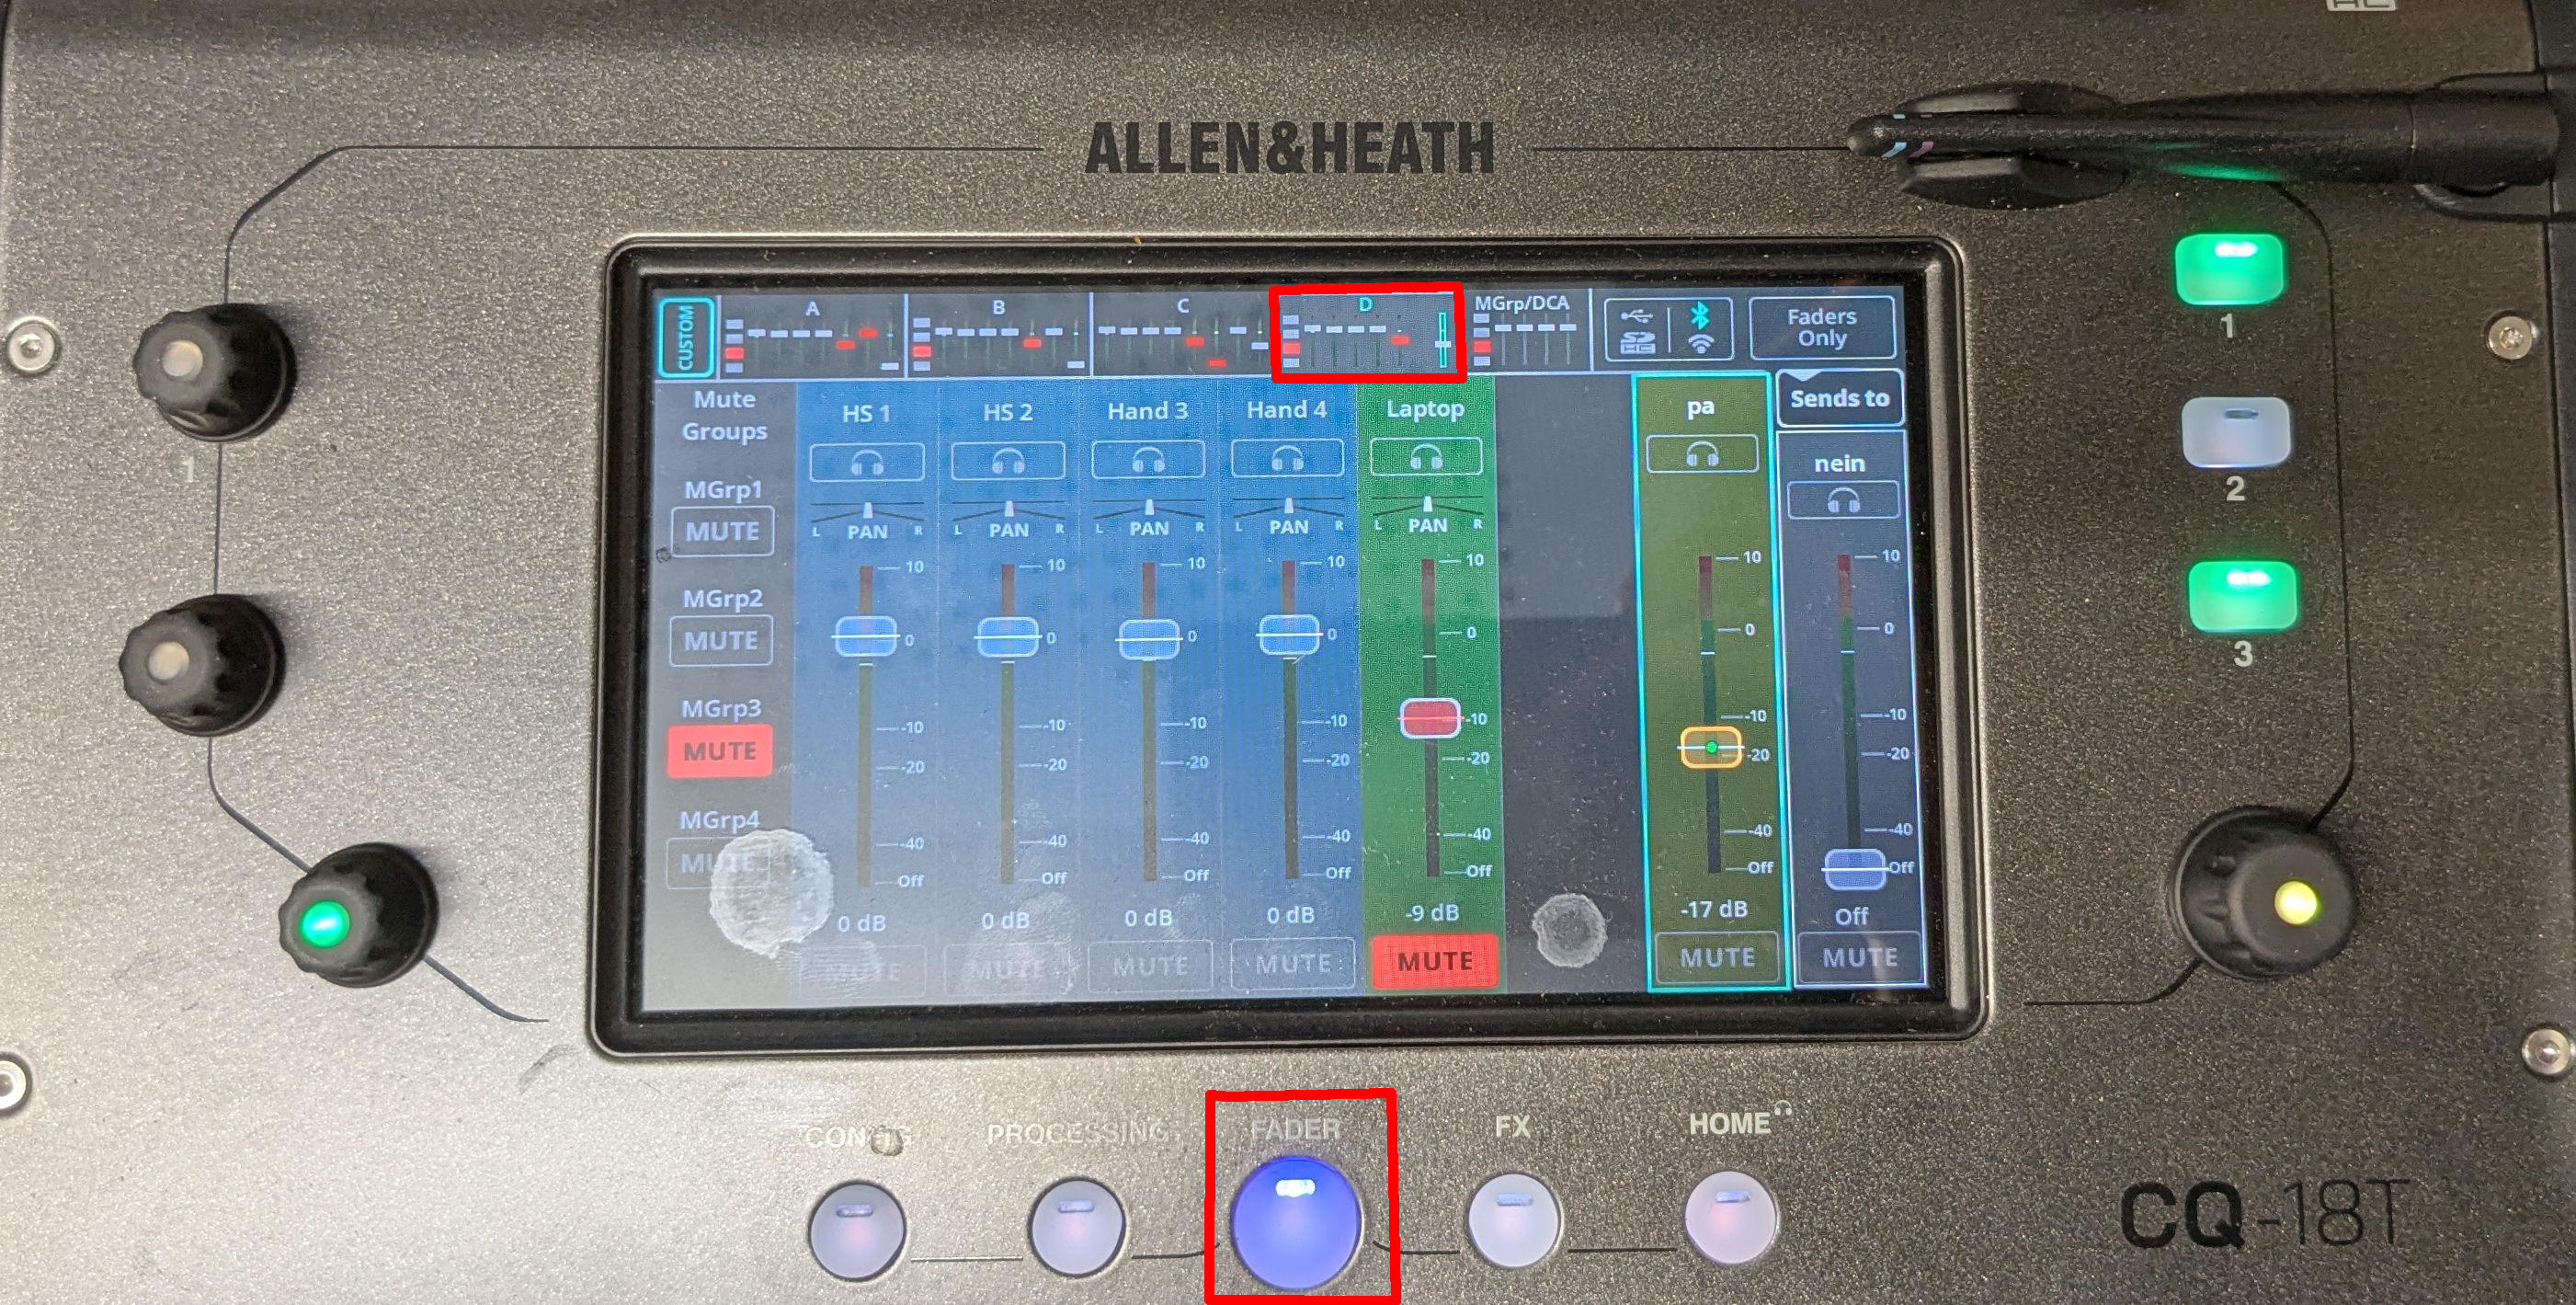
\includegraphics[width=0.9\textwidth]{images/allenheath-layers.jpg}
			\caption{Allen \& Heath CQ18T Layers}
		\end{figure}
		\column{0.4\textwidth}
		\begin{itemize}
			\item Please make sure, to always work on "Custom Workbench D"
			\item If anything else is shown, contact VOC or A/V-Technician before the talk
		\end{itemize}
	\end{columns}
\end{frame}

\begin{frame}{Audio Mixer Controls: Levels}
	\begin{columns}[T,onlytextwidth]
		\column{0.6\textwidth}
		\begin{figure} 
			\centering
			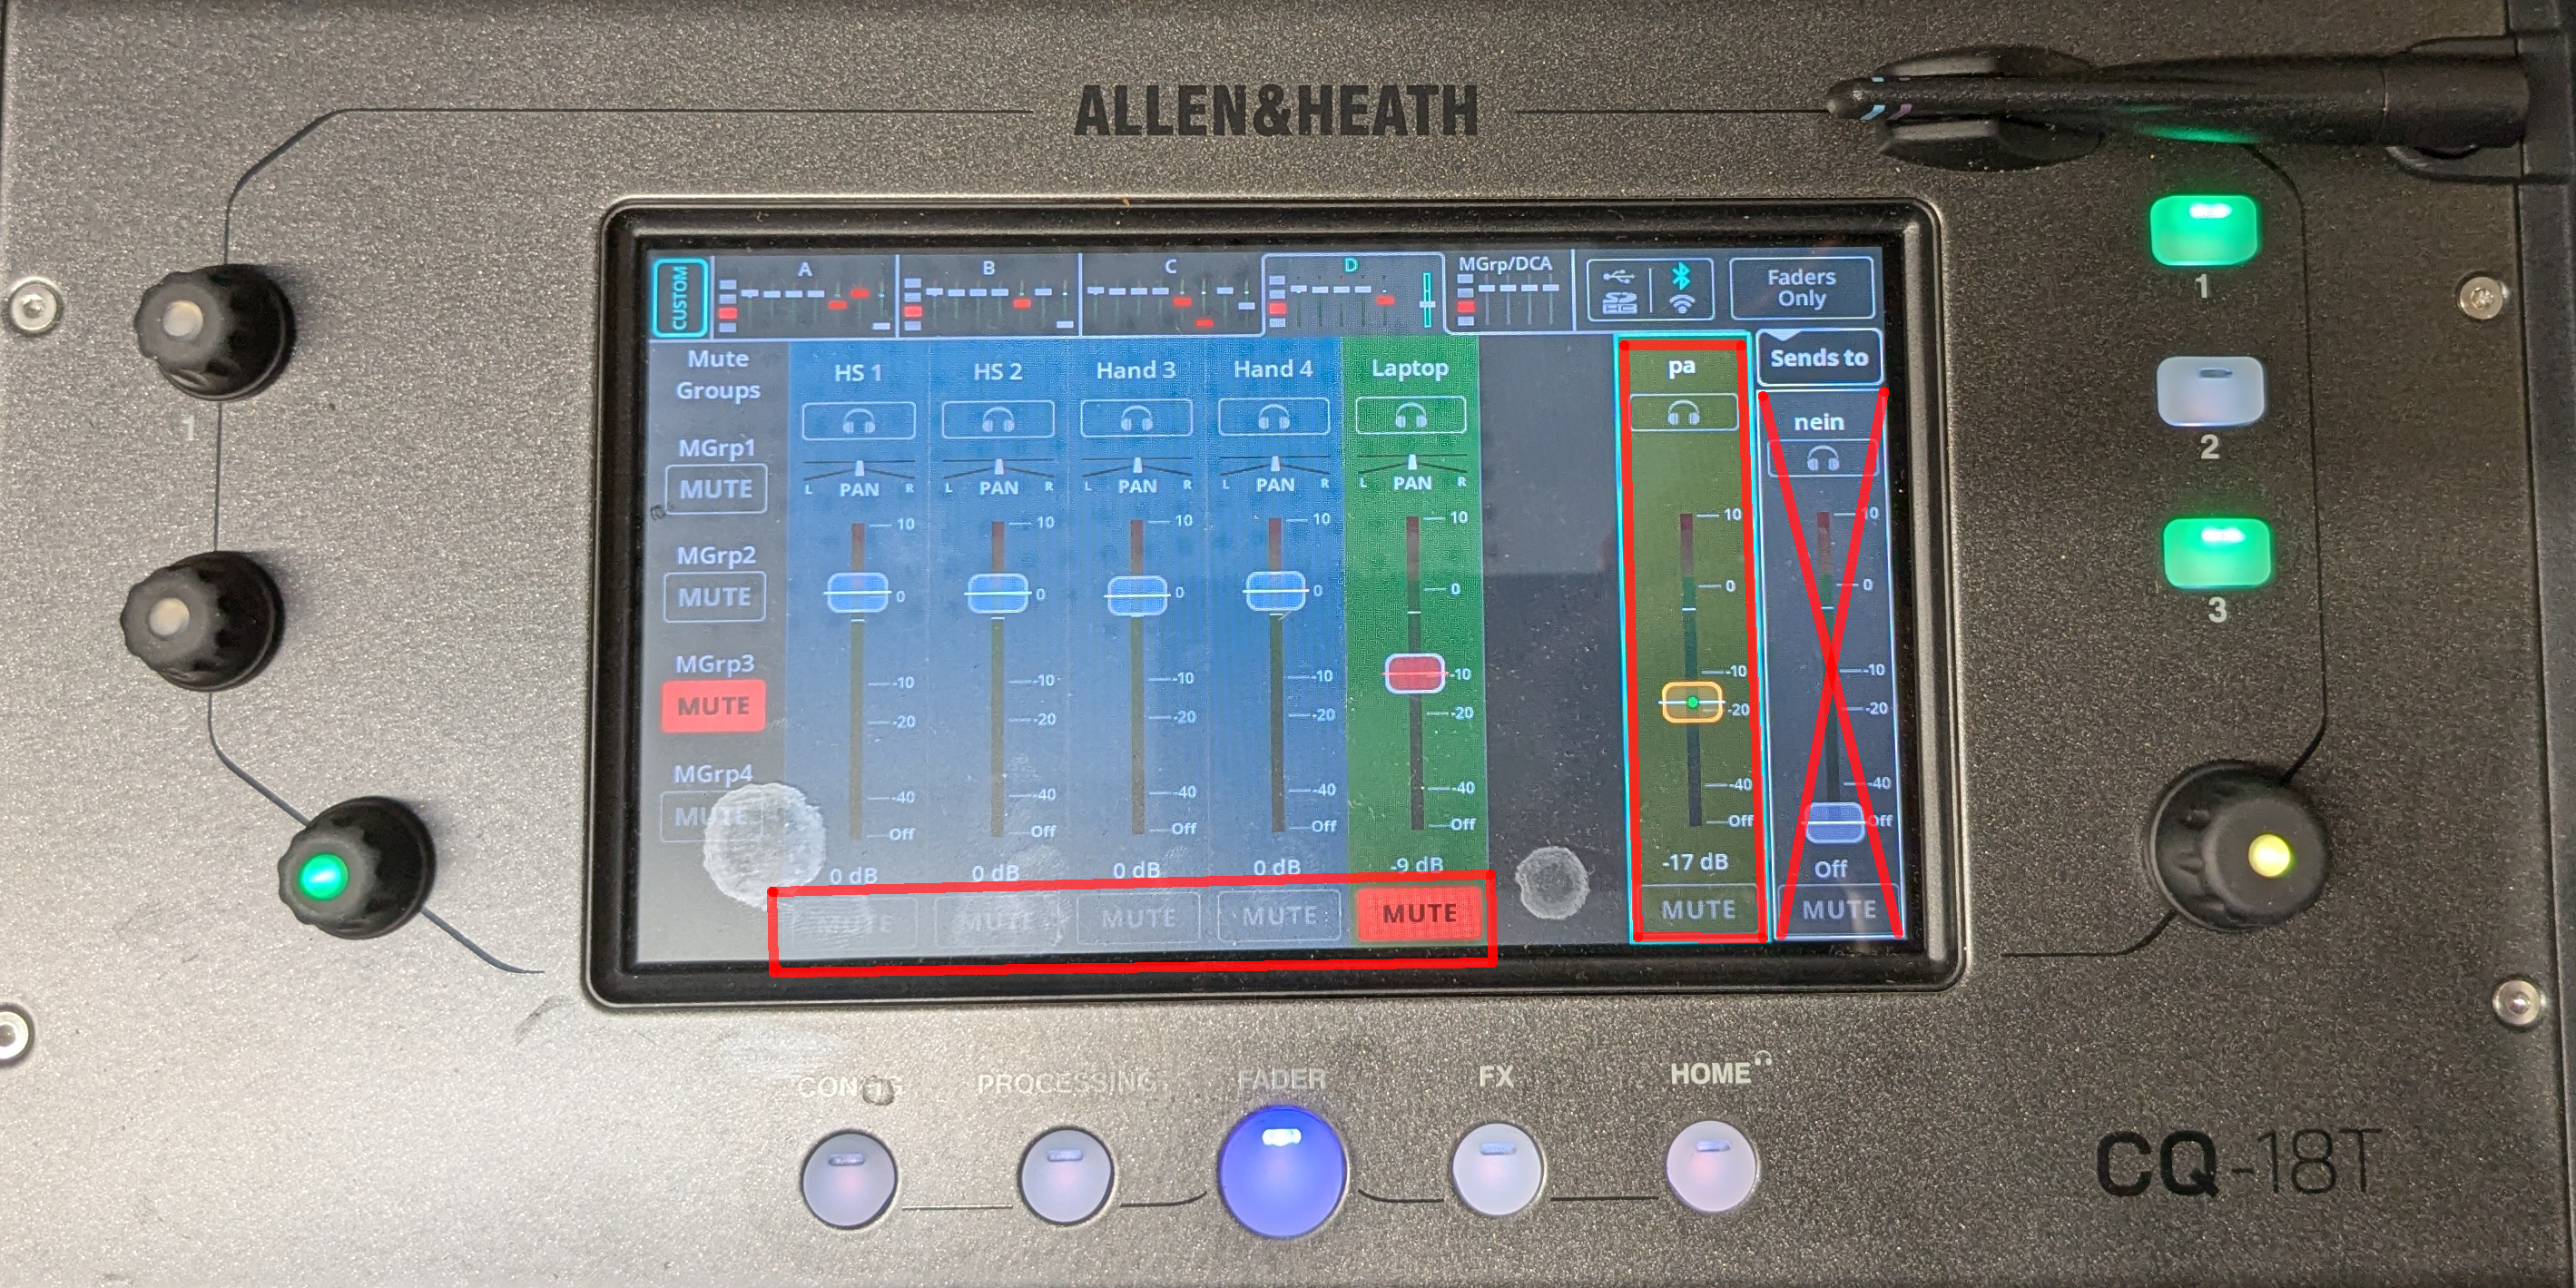
\includegraphics[width=0.9\textwidth]{images/allenheath-main-controls.jpg}
			\caption{Allen \& Heath CQ18T Main Controls}
		\end{figure}
		\column{0.4\textwidth}
		\begin{itemize}
			\item Mute unused microphones (bottom row)
			\item Adjust hall loudness with fader labeled "PA"
			\item Do not use the fader labeled "NEIN"
			\item Please keep microphones un-muted during applause
		\end{itemize}
	\end{columns}
\end{frame}
